\documentclass[11pt,a4paper]{article}

% Packages
\usepackage[utf8]{inputenc}
\usepackage[T1]{fontenc}
\usepackage[margin=2.5cm]{geometry}
\usepackage{amsmath,amssymb}
\usepackage{enumitem}
\usepackage{listings}
\usepackage{xcolor}
\usepackage{tikz}
\usetikzlibrary{shapes.geometric, arrows, positioning, calc}
\usepackage{fancyhdr}
\usepackage{lastpage}
\usepackage{array}
\usepackage{tabularx}
\usepackage{booktabs}

% Code listing style
\definecolor{codebg}{RGB}{248,248,248}
\definecolor{codeframe}{RGB}{200,200,200}
\definecolor{codekw}{RGB}{0,0,180}
\definecolor{codecomment}{RGB}{0,128,0}
\definecolor{codestring}{RGB}{163,21,21}

\lstdefinestyle{pythonstyle}{
    language=Python,
    basicstyle=\ttfamily\small,
    keywordstyle=\color{codekw}\bfseries,
    commentstyle=\color{codecomment}\itshape,
    stringstyle=\color{codestring},
    backgroundcolor=\color{codebg},
    frame=single,
    rulecolor=\color{codeframe},
    numbers=left,
    numberstyle=\tiny\color{gray},
    numbersep=8pt,
    showstringspaces=false,
    breaklines=true,
    tabsize=4,
    xleftmargin=15pt,
    framexleftmargin=15pt,
}

\lstset{style=pythonstyle}

% Flowchart styles
\tikzstyle{startstop} = [rectangle, rounded corners, minimum width=2.5cm, minimum height=0.8cm, text centered, draw=black, fill=red!20]
\tikzstyle{process} = [rectangle, minimum width=2.5cm, minimum height=0.8cm, text centered, draw=black, fill=blue!15]
\tikzstyle{decision} = [diamond, aspect=2, minimum width=2cm, minimum height=0.8cm, text centered, draw=black, fill=green!15]
\tikzstyle{io} = [trapezium, trapezium left angle=70, trapezium right angle=110, minimum width=2cm, minimum height=0.8cm, text centered, draw=black, fill=orange!15]
\tikzstyle{arrow} = [thick,->,>=stealth]

% Header and footer
\pagestyle{fancy}
\fancyhf{}
\lhead{Python Programming -- Intermediate Exam}
\rhead{Units 1--7}
\cfoot{Page \thepage\ of \pageref{LastPage}}

% Points box
\newcommand{\pointsbox}[1]{\hfill\fbox{\textbf{#1 pts}}}

\begin{document}

% Title section
\begin{center}
  {\Large\bfseries Python Programming \& Data Analysis}\\[0.3cm]
  {\large Intermediate Exam -- Units 1--7}\\[0.5cm]
  \begin{tabular}{|p{6cm}|p{6cm}|}
    \hline
    \textbf{Name:}       & \\[0.5cm]
    \hline
    \textbf{Student ID:} & \\[0.5cm]
    \hline
    \textbf{Date:}       & \\[0.5cm]
    \hline
  \end{tabular}
\end{center}

\vspace{0.5cm}

\noindent\textbf{Instructions:}
\begin{itemize}[noitemsep]
  \item Time allowed: \textbf{90 minutes}
  \item Total points: \textbf{105 points}
  \item No aids (no notes, no electronic devices)
  \item Write legibly; illegible answers may not be graded
  \item Show your work where applicable
\end{itemize}

\vspace{0.3cm}

\noindent\textbf{Points Summary:}
\begin{center}
  \begin{tabular}{|c|c|c|}
    \hline
    \textbf{Question} & \textbf{Max Points} & \textbf{Score} \\
    \hline
    1                 & 8                   &                \\
    \hline
    2                 & 12                  &                \\
    \hline
    3                 & 10                  &                \\
    \hline
    4                 & 12                  &                \\
    \hline
    5                 & 14                  &                \\
    \hline
    6                 & 12                  &                \\
    \hline
    7                 & 16                  &                \\
    \hline
    8                 & 21                  &                \\
    \hline
    \textbf{Total}    & \textbf{105}        &                \\
    \hline
  \end{tabular}
\end{center}

\newpage

%==============================================================================
% QUESTION 1: Multiple Choice (Fundamentals & Types)
%==============================================================================
\section*{Question 1: Multiple Choice \pointsbox{8}}

\textit{Circle the correct answer for each question. Each correct answer is worth 2 points.}

\vspace{0.4cm}

\begin{enumerate}[label=\textbf{1.\arabic*}]
  \item What is the output of the following expression?
        \begin{lstlisting}[numbers=none]
result = 17 // 5
print(result)
    \end{lstlisting}
        \begin{enumerate}[label=\Alph*)]
          \item \texttt{3.4}
          \item \texttt{3}
          \item \texttt{2}
          \item \texttt{17}
        \end{enumerate}

        \vspace{0.5cm}

  \item Which of the following is a \textbf{mutable} data structure in Python?
        \begin{enumerate}[label=\Alph*)]
          \item \texttt{tuple}
          \item \texttt{str}
          \item \texttt{list}
          \item \texttt{int}
        \end{enumerate}

        \vspace{0.5cm}

  \item What will \texttt{type(3.14)} return?
        \begin{enumerate}[label=\Alph*)]
          \item \texttt{<class 'int'>}
          \item \texttt{<class 'float'>}
          \item \texttt{<class 'str'>}
          \item \texttt{<class 'number'>}
        \end{enumerate}

        \vspace{0.5cm}

  \item In Python, what does the keyword \texttt{self} represent in a class method?
        \begin{enumerate}[label=\Alph*)]
          \item The class itself
          \item The parent class
          \item The current instance/object
          \item A global variable
        \end{enumerate}
\end{enumerate}

\newpage

%==============================================================================
% QUESTION 2: Predict the Output
%==============================================================================
\section*{Question 2: Predict the Output \pointsbox{12}}

\textit{For each code snippet, write exactly what will be printed. Be precise with spacing and format. Each answer is worth 3 points.}

\vspace{0.4cm}

\begin{enumerate}[label=\textbf{2.\arabic*}]
  \item \textbf{(3 pts)}
        \begin{lstlisting}
numbers = [10, 20, 30, 40, 50]
print(numbers[1:4])
print(numbers[-2])
    \end{lstlisting}
        \textbf{Output:}
        \vspace{2.5cm}

  \item \textbf{(3 pts)}
        \begin{lstlisting}
x = 5
y = 3
x, y = y, x + y
print(f"x={x}, y={y}")
    \end{lstlisting}
        \textbf{Output:}
        \vspace{2.5cm}

  \item \textbf{(3 pts)}
        \begin{lstlisting}
data = {"a": 1, "b": 2, "c": 3}
for key in data:
    if data[key] > 1:
        print(key, end=" ")
    \end{lstlisting}
        \textbf{Output:}
        \vspace{2.5cm}

  \item \textbf{(3 pts)}
        \begin{lstlisting}
def process(items):
    items.append(4)
    items = [100]
    return items

original = [1, 2, 3]
result = process(original)
print(original)
print(result)
    \end{lstlisting}
        \textbf{Output:}
        \vspace{2.5cm}
\end{enumerate}

\newpage

%==============================================================================
% QUESTION 3: Find the Errors
%==============================================================================
\section*{Question 3: Find and Fix the Errors \pointsbox{10}}

\textit{Each code snippet contains one or more errors. Identify each error and write the corrected line(s). Explain briefly what was wrong.}

\vspace{0.4cm}

\begin{enumerate}[label=\textbf{3.\arabic*}]
  \item \textbf{(3 pts)} The following code should print ``Hello, World!'' but contains an error:
        \begin{lstlisting}
message = "Hello, World!
print(message)
    \end{lstlisting}
        \textbf{Error:} \hrulefill \\[0.3cm]
        \textbf{Correction:} \hrulefill \\[0.8cm]

  \item \textbf{(4 pts)} The following function should return the sum of all numbers in a list:
        \begin{lstlisting}
def sum_list(numbers)
    total = 0
    for num in numbers:
    total += num
    return total
    \end{lstlisting}
        \textbf{Errors (list all):} \\[0.5cm]
        \hrulefill \\[0.3cm]
        \hrulefill \\[0.3cm]
        \hrulefill \\[0.5cm]
        \textbf{Corrected code:} \\[4cm]

  \item \textbf{(3 pts)} The following class definition has an error:
        \begin{lstlisting}
class Dog:
    def __init__(name, breed):
        self.name = name
        self.breed = breed

dog1 = Dog("Buddy", "Labrador")
    \end{lstlisting}
        \textbf{Error:} \hrulefill \\[0.3cm]
        \textbf{Correction:} \hrulefill
\end{enumerate}

\newpage

%==============================================================================
% QUESTION 4: Flowchart to Code
%==============================================================================
\section*{Question 4: Flowchart to Python Code \pointsbox{12}}

\textit{Study the following flowchart and write the equivalent Python code. The flowchart takes a positive integer and produces a result based on extracting and processing its digits.}

\vspace{0.4cm}

\begin{center}
  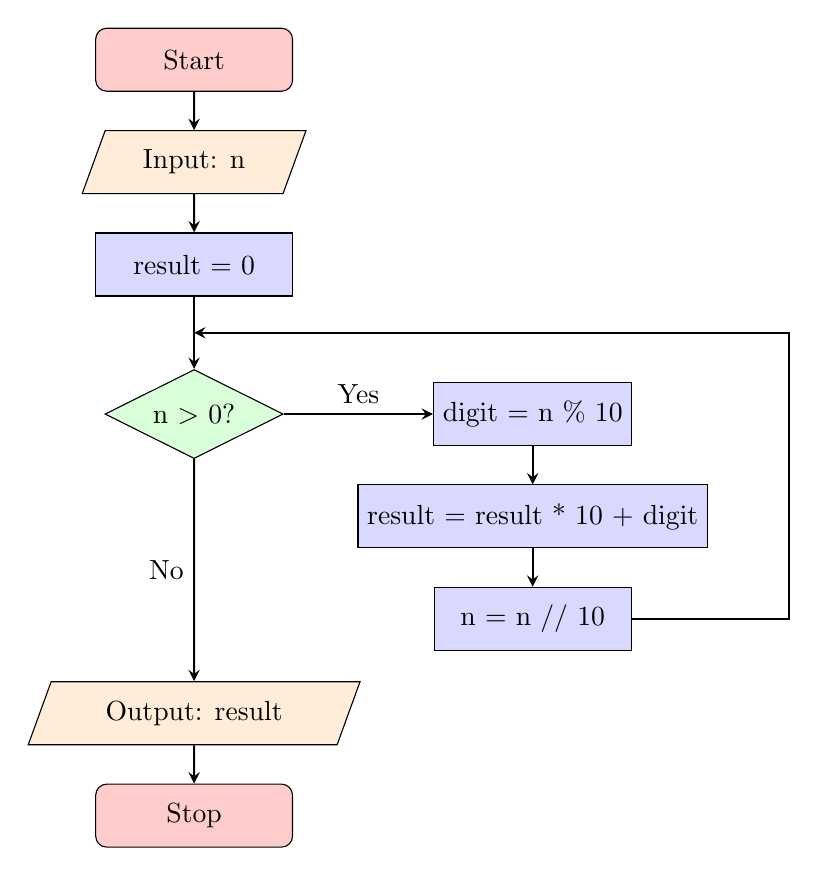
\begin{tikzpicture}[node distance=1.3cm]
    \node (start) [startstop] {Start};
    \node (input) [io, below of=start] {Input: n};
    \node (init) [process, below of=input] {result = 0};
    \node (check) [decision, below of=init, yshift=-0.6cm] {n $>$ 0?};
    \node (getdigit) [process, right of=check, xshift=3cm] {digit = n \% 10};
    \node (build) [process, below of=getdigit] {result = result * 10 + digit};
    \node (reduce) [process, below of=build] {n = n // 10};
    \node (output) [io, below of=check, yshift=-2.5cm] {Output: result};
    \node (stop) [startstop, below of=output] {Stop};

    \draw [arrow] (start) -- (input);
    \draw [arrow] (input) -- (init);
    \draw [arrow] (init) -- (check);
    \draw [arrow] (check) -- node[anchor=south] {Yes} (getdigit);
    \draw [arrow] (getdigit) -- (build);
    \draw [arrow] (build) -- (reduce);
    % Loop back: go right, then up, then left to join the line between init and check
    \coordinate (loopback) at ($(init.south)!0.5!(check.north)$);
    \draw [arrow] (reduce.east) -- +(2,0) |- (loopback);
    \draw [arrow] (check) -- node[anchor=east] {No} (output);
    \draw [arrow] (output) -- (stop);
  \end{tikzpicture}
\end{center}

\vspace{0.3cm}
\textbf{Hint:} Trace through the flowchart with \texttt{n = 123} to understand what it does before writing the code.

\vspace{0.2cm}
\textbf{Reminder:} \texttt{\%} gives the remainder, \texttt{//} gives the integer quotient.\\
\textit{Example:} \texttt{47 \% 10 = 7} \quad and \quad \texttt{47 // 10 = 4}

\vspace{0.3cm}

\textbf{Write the Python code that implements this flowchart:}

\vspace{8cm}

\newpage

%==============================================================================
% QUESTION 5: Code to Flowchart
%==============================================================================
\section*{Question 5: Python Code to Flowchart \pointsbox{14}}

\textit{Given the following Python code, draw a flowchart that represents its logic. Use proper flowchart symbols (oval for start/stop, rectangle for process, diamond for decision, parallelogram for input/output).}

\vspace{0.4cm}

\begin{lstlisting}
def analyze_grades(grades):
    if len(grades) == 0:
        return "No grades", 0, 0
    
    total = 0
    passed = 0
    
    for grade in grades:
        total = total + grade
        if grade >= 50:
            passed = passed + 1
    
    average = total / len(grades)
    
    if average >= 70:
        status = "Excellent"
    elif average >= 50:
        status = "Passed"
    else:
        status = "Failed"
    
    return status, average, passed
\end{lstlisting}

\vspace{0.5cm}

\textbf{Draw your flowchart below:}

\vspace{14cm}

\newpage

%==============================================================================
% QUESTION 6: Data Structures
%==============================================================================
\section*{Question 6: Data Structures \pointsbox{12}}

\begin{enumerate}[label=\textbf{6.\arabic*}]
  \item \textbf{(4 pts)} Given the following dictionary, write Python code to:
        \begin{lstlisting}[numbers=none]
students = {
    "Alice": 85,
    "Bob": 72,
    "Charlie": 91,
    "Diana": 68
}
    \end{lstlisting}

        \begin{enumerate}[label=\alph*)]
          \item Add a new student ``Eve'' with grade 88: \\[0.8cm]
                \hrulefill \\[0.5cm]

          \item Print all students who scored above 80: \\[0.5cm]
                \hrulefill \\[0.3cm]
                \hrulefill \\[0.3cm]
                \hrulefill \\[0.3cm]
                \hrulefill \\[0.5cm]
        \end{enumerate}

  \item \textbf{(4 pts)} What is the difference between a \textbf{list} and a \textbf{tuple}? Give one practical use case for each. \\[0.5cm]
        \hrulefill \\[0.3cm]
        \hrulefill \\[0.3cm]
        \hrulefill \\[0.3cm]
        \hrulefill \\[0.3cm]
        \hrulefill \\[0.3cm]
        \hrulefill \\[0.5cm]

  \item \textbf{(4 pts)} What will be the contents of \texttt{my\_set} after executing the following code?
        \begin{lstlisting}
my_set = {1, 2, 3, 2, 4, 1, 5, 3}
my_set.add(6)
my_set.add(2)
my_set.remove(4)
    \end{lstlisting}
        \textbf{Answer:} \hrulefill \\[0.3cm]
        \hrulefill
\end{enumerate}

\newpage

%==============================================================================
% QUESTION 7: Functions
%==============================================================================
\section*{Question 7: Functions \pointsbox{16}}

\begin{enumerate}[label=\textbf{7.\arabic*}]
  \item \textbf{(6 pts)} Complete the following function that takes a list of numbers and returns a new list containing only the even numbers:
        \begin{lstlisting}
def filter_even(numbers):
    # Your code here
    
    
    
    
    
    
    
    
    \end{lstlisting}

  \item \textbf{(4 pts)} Explain the difference between these two functions. What will each print when called?
        \begin{lstlisting}
def func_a(x):
    print(x * 2)

def func_b(x):
    return x * 2

result_a = func_a(5)
result_b = func_b(5)
print(f"result_a: {result_a}")
print(f"result_b: {result_b}")
    \end{lstlisting}
        \textbf{Explanation and Output:} \\[0.3cm]
        \hrulefill \\[0.3cm]
        \hrulefill \\[0.3cm]
        \hrulefill \\[0.3cm]
        \hrulefill \\[0.3cm]
        \hrulefill \\[0.3cm]
        \hrulefill \\[0.5cm]

  \item \textbf{(6 pts)} Write a function called \texttt{count\_vowels} that takes a string and returns the number of vowels (a, e, i, o, u) in it. The function should work for both uppercase and lowercase letters.

        \textbf{Example:} \texttt{count\_vowels("Hello World")} should return \texttt{3}

        \vspace{7cm}
\end{enumerate}

\newpage

%==============================================================================
% QUESTION 8: Object-Oriented Programming
%==============================================================================
\section*{Question 8: Object-Oriented Programming \pointsbox{21}}

\begin{enumerate}[label=\textbf{8.\arabic*}]
  \item \textbf{(5 pts)} What is the output of the following code? Explain why.
        \begin{lstlisting}
class ProgressTracker:
    def __init__(self, total_steps):
        self._total = total_steps
        self._completed = 0
    
    @property
    def completed(self):
        return self._completed
    
    @completed.setter
    def completed(self, value):
        if value < 0:
            self._completed = 0
        elif value > self._total:
            self._completed = self._total
        else:
            self._completed = value
    
    @property
    def percentage(self):
        return (self._completed / self._total) * 100

tracker = ProgressTracker(10)
tracker.completed = 7
print(tracker.percentage)
tracker.completed = 15
print(tracker.completed)
print(tracker.percentage)
    \end{lstlisting}
        \textbf{Output:} \\[0.3cm]
        \hrulefill \\[0.3cm]
        \hrulefill \\[0.3cm]
        \hrulefill \\[0.5cm]
        \textbf{What is the purpose of the setter validation in this code?} \\[0.3cm]
        \hrulefill \\[0.3cm]
        \hrulefill \\[0.8cm]

        \newpage
  \item \textbf{(5 pts)} The following code has a common OOP bug. Identify the bug, explain why it happens, and write the corrected code.
        \begin{lstlisting}
class ChatRoom:
    messages = []
    
    def __init__(self, room_name):
        self.room_name = room_name
    
    def post_message(self, user, text):
        self.messages.append(f"{user}: {text}")

room1 = ChatRoom("General")
room2 = ChatRoom("Sports")
room1.post_message("Alice", "Hello!")
room2.post_message("Bob", "Goal!")
print(f"General: {room1.messages}")
print(f"Sports: {room2.messages}")
    \end{lstlisting}
        \textbf{What is the bug and why does it happen?} \\[0.3cm]
        \hrulefill \\[0.3cm]
        \hrulefill \\[0.3cm]
        \hrulefill \\[0.5cm]
        \textbf{Write the corrected \texttt{\_\_init\_\_} method:} \\[2.5cm]

        \newpage

  \item \textbf{(6 pts)} Complete the \texttt{Playlist} class with proper encapsulation. The songs list should be private (use \texttt{\_songs}) and only accessible through a property that returns a copy (to prevent external modification).
        \begin{lstlisting}
class Playlist:
    def __init__(self, name):
        self.name = name
        # TODO: Initialize private _songs as empty list
        
    
    @property
    def songs(self):
        # TODO: Return a COPY of the songs list
        
    
    @property
    def count(self):
        # TODO: Return number of songs
        
    
    def add_song(self, title):
        # TODO: Add song only if not already in playlist
        # Return True if added, False if duplicate
        
        
        
        
    
    def remove_song(self, title):
        # TODO: Remove song if exists
        # Return True if removed, False if not found
        
        
        
        
        
    \end{lstlisting}

        \newpage
  \item \textbf{(5 pts)} Consider the following inheritance hierarchy:
        \begin{lstlisting}
class Notification:
    def __init__(self, message):
        self.message = message
    
    def send(self):
        return f"Sending: {self.message}"

class EmailNotification(Notification):
    def __init__(self, message, recipient):
        super().__init__(message)
        self.recipient = recipient
    
    def send(self):
        base = super().send()
        return f"{base} to {self.recipient}"

class UrgentEmail(EmailNotification):
    def send(self):
        return "[URGENT] " + super().send()

notif = UrgentEmail("Server down!", "admin@example.com")
print(notif.send())
print(isinstance(notif, Notification))
    \end{lstlisting}

        \begin{enumerate}[label=\alph*)]
          \item What will be printed? \\[0.3cm]
                \hrulefill \\[0.3cm]
                \hrulefill \\[0.5cm]

          \item Trace the \texttt{super().send()} calls: which methods are called and in what order when \texttt{notif.send()} executes? \\[0.3cm]
                \hrulefill \\[0.3cm]
                \hrulefill \\[0.3cm]
                \hrulefill \\[0.5cm]

          \item Why does \texttt{UrgentEmail} not need its own \texttt{\_\_init\_\_} method? \\[0.3cm]
                \hrulefill \\[0.3cm]
                \hrulefill
        \end{enumerate}
\end{enumerate}

\vspace{1cm}

\begin{center}
  \rule{8cm}{0.4pt}\\[0.3cm]
  \textbf{End of Exam}\\[0.2cm]
  \textit{Good luck!}
\end{center}

\end{document}
